\documentclass[12pt,twoside]{report}
\relpenalty=9999
\binoppenalty=9999
%\documentclass[12pt,preprint]{}
\usepackage[utf8]{inputenc}
\usepackage{graphicx}
\graphicspath{{images/}}
\usepackage{caption}
\usepackage{subcaption}
\usepackage[a4paper,width=150mm,top=25mm,bottom=25mm]{geometry}
\usepackage{fancyhdr}
\usepackage{amsbsy}
\usepackage{amsmath}


\usepackage[multidot]{grffile}%dots in graphics file names
\usepackage{multicol}%split equations for SAFT into two columns

\pagestyle{fancy}
\fancyhead{}
\fancyhead[RO,LE]{Finding the arbitrary parameter L in Renormalization Group Theory via fitting Monte Carlo simulations to Statistical Associating Fluid Theory}
\fancyfoot{}
\fancyfoot[LE,RO]{\thepage}
\fancyfoot[LO,CE]{Chapter \thechapter}
\fancyfoot[CO,RE]{Billy Edward Geerhart III}
\renewcommand{\headrulewidth}{0.4pt}
\renewcommand{\footrulewidth}{0.4pt}

\usepackage[backend=bibtex,maxnames=99,sorting=none]{biblatex}
\addbibresource{references.bib}



%????
\iffalse
\usepackage{etoolbox}% http://ctan.org/pkg/etoolbox
\makeatletter
% \patchcmd{<cmd>}{<search>}{<replace>}{<success>}{<failure>}
% --- Patch \chapter
%\patchcmd{\@makechapterhead}{50\p@}{\chapheadtopskip}{}{}% Space from top of page to CHAPTER X
\patchcmd{\@makechapterhead}{50\p@}{\chapheadtopskip}{}{}

%\patchcmd{\@makechapterhead}{20\p@}{\chapheadsep}{}{}% Space between CHAPTER X and CHAPTER TITLE
\patchcmd{\@makechapterhead}{20\p@}{\chapheadsep}{}{}

%\patchcmd{\@makechapterhead}{40\p@}{\chapheadbelowskip}{}{}% Space between CHAPTER TITLE and text
\patchcmd{\@makechapterhead}{40\p@}{\chapheadbelowskip}{}{}

% --- Patch \chapter*
%\patchcmd{\@makeschapterhead}{50\p@}{\chapheadtopskip}{}{}% Space from top of page to CHAPTER TITLE
\patchcmd{\@makeschapterhead}{10\p@}{\chapheadtopskip}{}{}

%\patchcmd{\@makeschapterhead}{40\p@}{\chapheadbelowskip}{}{}% SPace between CHAPTER TITLE and text
\patchcmd{\@makeschapterhead}{0\p@}{\chapheadbelowskip}{}{}
\makeatother
% Set new lengths
\newlength{\chapheadtopskip}\setlength{\chapheadtopskip}{0pt}
\newlength{\chapheadsep}\setlength{\chapheadsep}{0pt}
\newlength{\chapheadbelowskip}\setlength{\chapheadbelowskip}{1pt}
\fi
% end ????

%???  changes chapter headings
\usepackage{titlesec}

%\titleformat{\chapter}[display]{\normalfont\huge\bfseries}{\thechapter.}{0pt}{\huge\it}
%\titlespacing*{\chapter}{0pt}{0pt}{1pt}
\titleformat{\chapter}[display]
{\normalfont\huge\bfseries}{}{-50pt}{\Huge}
\titlespacing*{\chapter} {0pt}{-50pt}{0pt}
%  end %%%%


%\title{
%	{Exploring Phase Equilibrium with Statistical non-Associating Fluid Theory}\\
%	{\large Oregon State University}\\
%	{
\includegraphics{osu2.PNG}}
%	}


\title{Finding the arbitrary parameter L in Renormalization Group Theory VIA fitting Monte Carlo simulations to Statistical Associating Fluid Theory}

\author{Billy Edward Geerhart III}
%\date{\today}
\begin{document}


\begin{titlepage}
	\begin{center}
	\vspace*{1cm}
	
	\Huge
	\textbf{Finding the arbitrary parameter L in Renormalization Group Theory}
	
	\vspace{0.5cm}
	\LARGE
	 VIA fitting Monte Carlo simulations to Statistical Associating Fluid Theory
	
	\vspace{1.5cm}
	
	\textbf{Billy Edward Geerhart III}
	
	\vfill
	
	A project presented for the degree of\\
	Masters of Science
	
	\vspace{0.8cm}
	
	
\includegraphics{osu2}
	
	\Large
	Department of Physics\\
	Oregon State University\\
	\today
	
	\end{center}
\end{titlepage}

%\maketitle

\thispagestyle{plain}
\begin{center}
	\Large
	\textbf{Exploring Phase Equilibrium with Statistical non-Associating Fluid Theory:}
	
	\vspace{0.4cm}
	\large
	A Generalized Renormalization Group Theory Approach.
	
	\vspace{0.4cm}
	\textbf{Ryan M. Scheirer}
	
	\vspace{0.9cm}
	\textbf{Abstract}
\end{center}

Abstract goes hereeee!


\tableofcontents

\listoffigures

\chapter{Introduction}
%\section{Introduction}
\begin{figure}[h]
\vspace*{-0mm}
\hspace*{-6mm}
	\centering
	\includegraphics[width=\textwidth]{renorm}
	\caption{
	%\tiny	
	\scriptsize
	Here a simulation of a 2d fluid near the critical point is presented. The three images are the same fluid seperated in time. The interface between liquid and gas evolves in time as each globule will interact with neighboring globules. If the temperature is increased past the critical point, the globules shrink in size to the point the plots appear as white noise.}
	\label{fig:renorm}
\end{figure}

The liquid-vapor phase coexistence can be found by just placing some liquid into a sealed container. Some of the liquid will evaporate into the jar creating a vapor pressure. Provided we placed enough liquid into the jar, the system will now contain both a liquid and a vapor at the same time. By sealing the liquid into a jar, we have forced the pressure of the liquid to be the as the pressure of the gas. By allowing the atoms to swap between the liquid and gas phase, we have also allowed the chemical potential of the liquid to be the same as that of the gas.

Although we can find the phase coexistence by physically sealing a liquid in a jar, an equivalent computational method is to use an empirically determined fluid model which we can use to run simulations that also equalize the pressur
e and chemical potential. The problem with the computational method is the empirical model requires fitting a few parameters to data, data which probably already includes points on the phase coexistence curve. The main benefit to the computational approach is that once the empirical parameters are found, we can then create the phase coexistence of a mixture of fluids using the previously determined parameters.

One of the difficulties with the computer simulations is computation time. A simulation with a handful of atoms can be finished within 20 minutes, yet a simulation with a 100 atoms can take as long as 4 days. To recreate the phase coexistence graph requires setting the pressure and chemical potential of both phases equal to each other, but this is equivalent to plotting the free energy as a function of density and searching for a common cotangent. For even a simulation that uses a small box, the problem is plotting free energy as a function of density requires many simulations at various densities; some simulations containing only a handful of atoms while other simulations containing as much as a couple hundred atoms. Total computation time for 10 computer cores to create the free energy as a function of density graph can take as long as three weeks.

Naturally there is a tradeoff between a realistic computation time for a project and how realistic the results are going to be. The simulations use periodic boundary conditions which is just the thermodynamic way of saying the boundary should not affect the bulk properties. The key part being whatever is in the simulation is considered the bulk, which is a problem since a small simulation can hardly be considered the bulk. To get around this problem, the simulation size is usually increased until the simulation does represent the bulk. 

Normally increasing the simulation size is just fine, but there is a regime where the bulk properties depend on length scales of the order of a millimeter. This regime occurs near the critical point where the liquid density approaches that of the vapor. Normally the liquid and vapor are entirely seperated due to the surface tension. However; as the system approaches the critical point, the surface tension approaches zero which means the liquid and vapor will start to mix. Although figure 1 shows an extreme example of a liquid completely mixing with vapor, even under normal circumstances there exist natural fluctuations in the density of either phase. It just so happens that these fluctuations are significant as the density of the liquid approaches the density of the gas at the critical point. Basically the fluctuations within each phase would normally be rather small, but near the critical point the fluctuations are relatively big since the gas and liquid phases are morphing into each other. This is a problem since it requires the simulations to be about the same size as that of the largest fluctuation. For example, a 1mm length box would contain roughly $10^{19}$ atoms, which would require an unfeasible computation time.

Renormalization group theory(RGT) can be applied to get around this large fluctuation problem. Simply put, RGT is a method in which fine details are omitted from calculations while still maintaining accuracy. This is done by transforming the original partition funciton into a smaller partition function, but the smaller system is renormalized to the original parition function. [add details...]

In particular, RGT is applied through an interaction wave length. The zeroth order is just the ideal gas term in which all atoms only interact with the walls of the enclosure. The next order is applied via SAFT-VR in which a mean interaction and an approximate wavelength interaction is applied. Longer wavelength interactions can then be applied using RGT via a iterative method that steadily increases the size of the box.

The main problem this project addresses is the transition from SAFT-VR to the application of RGT. Within RGT there is an arbitrary base wavelength L which is usually fit to the data. However; this arbitrary wavelength shouldn't really be an arbitrary parameter as SAFT-VR already includes interactions at some unknown wavelength. This project attempts to find the base wavelength that SAFT-VR implements, and tests how the results of RGT change when using this base wavelength.

The base wavelength is found by using Monte Carlo Markov Chain (MCMC) simulations at various box sizes. The idea is that a MCMC simulation using a fixed box size of $L_0$ will incorporate interactions at this box size. The box size is then varied until the results from the MCMC simulations fit the results from SAFT-VR. Once the optimal box size is found, RGT is implemented using this optimal box size and the results are compared to previous results.



\chapter{Methods}
%\section{}
%\pagestyle{plain}   %Use if you do not want the fancy headers and footers... 
					 %({plain} -> just page number, {empty} -> nothing)...
					 % this will change all pages that come after this tex file...
					 % so make sure to reset the pagestyle to {fancy} at the end of this file
\newcommand\numberthis{\addtocounter{equation}{1}\tag{\theequation}}
The methods section is partitioned into theory, which define the equations used, and the actual implementation through computational techniques. The main point of the theory is to estimate the free energy F from which any of the thermodynamic variables can be found. For example, the entropy, checmical potential, pressure, or internal energy can be found by the following:
\begin{equation}
dF=-S\cdot dT -P\cdot dV+\mu\cdot dN
\end{equation}
\begin{equation}U=F+T\cdot S 
\end{equation} 
Once the free energy is found, the next goal is to fit the Monte Carlo simulations to SAFT by using a cost function that compares each thermodynamic variable from the Monte Carlo simulations to SAFT. The comparisons are constrained to a temperature range of $0.45<T/T_c<1.13$ where $T_c$ is the critical point using SAFT; the lower bound is chosen mostly to decrease the computation time of the simulations, while the upper limit is chosen to stay away from the well known hard sphere behavior. To decrease computation times even further, the comparisons are again constrained to filling fractions of [0.15,0.25,0.35,0.45]. Once the cost can be determined for a variety of box sizes, a 'best' box size is chosen that decreases the overall cost. The final step is to compare this best box size to slightly larger and smaller box sizes by looking at the coexistence densities of the liquid and gas phases.
\section{Fluid Model}
\begin{multicols}{2}
Molecular Dynamics
\begin{equation}
V_{Lennard-Jones}=4\epsilon\left[\left(\frac{\sigma}{4}\right)^{12}-\left(\frac{\sigma}{r}\right)^6\right]
\end{equation}
\\
Statistical Mechanics
\begin{equation}
V_{HardSphere}(r) =  
\begin{cases} 
 \infty &\text{if }r<sigma\\
 -\epsilon &\text{if }\sigma\leq r \leq \lambda\cdot\sigma \\
 0 & \text{otherwise}
\end{cases}
\end{equation}
\end{multicols}
Molecular dynamics usually simulates a fluid using a continuous potential that is used in combination with Newtonian mechanics. One common potential used is the Lennard-Jones potential; a potential which simulates a very strong repulsion at roughly $r=\sigma$, contains a finite well, and then tapers off to zero interaction as $r\rightarrow\infty$. On the other hand, Statistical Mechanics can even use the simpler hard sphere potential which also has a very strong repulsion at $r=\sigma$, has a finite well, and has zero interaction for very large $r$. The similarities between both methods is the actual dynamics of a real system is replaced with a computational fluid model that only attempts to match the boundary conditions of the actual fluids potential. Despite such a crude approximation, useful predictions can be made by empirically determining the parameters and using the model to extrapolate beyond the original experiments.

This project uses the hard sphere fluid in combination with statistical mechanics. The parameters used are $\sigma=2$ and $\lambda=1.5$.
\pagebreak
\section{Equation Summary: SAFT  }
Statistical Associating Fluid theory (SAFT) is a perturbation which attempts to model monomer interactions, directional interactions such as monomers binding into chains, and even chains interacting with themselves\cite{gil1997statistical}. The following equations are the square-well fluid results obtained by Gil-Villegas et al. \cite{gil1997statistical}:

\begin{multicols}{2}
let $n=\frac{N}{V}\newline\eta=packingFraction\newline\Lambda=$de Broglie wavlength

%gil-villegas eq. 1+18
\begin{equation}\label{eq:saftF18}
\frac{F}{N\cdot k\cdot T}=a^{IDEAL}+a^{HS}+\beta\cdot a_1^{SW}+\beta^2\cdot a_2^{SW}
\end{equation}

%gil-villegas eq 1
\begin{equation}\label{eq:saftF1a}
a^{IDEAL}=\ln\left(n\cdot \Lambda^3\right)-1
\end{equation}

%gil-villegas eq. 1
\begin{equation}\label{eq:saftF1b}
a^{HS}=-\ln(1-4\cdot \eta)
\end{equation}

%gil-villegas eq 34
\begin{equation}\label{eq:saftF34}
a_1^{SW}=a_1^{VDW}\cdot g^{HS}(1;\eta_{eff})
\end{equation}

%gil-villegas eq 35
\begin{equation}\label{eq:saftF35}
a_1^{VDW}=-4\cdot \eta\cdot \epsilon\cdot (\lambda^3-1)
\end{equation}

%gil-villegas eq 33
\begin{equation}\label{eq:saftF33}
g^{HS}(1;\eta_{eff})=\frac{1-\eta_{eff}/2}{(1-\eta_{eff})^3}
\end{equation}

%gil-villegas eq 36
\begin{equation}\label{eq:saftF36}
n_{eff}=c1\cdot \eta+c_2\cdot \eta^2+c_3\cdot \eta^3
\end{equation}

%gil-villegas eq 37
\begin{equation}\label{eq:saftF37}
\scriptscriptstyle
\begin{pmatrix}c_1\\c_2\\c_3\end{pmatrix}=
\begin{pmatrix}
2.25855 & -1.50349 & 0.249434 \\
-0.669270 & 1.40049 & -0.827739 \\
10.1576 & -15.0427 & 5.30827
\end{pmatrix}\times
\begin{pmatrix}
1\\ \lambda \\ \lambda^2
\end{pmatrix}
\end{equation}

%gil-villegas eq 38
\begin{equation}\label{eq:saft38}
a_2^{SW}=\frac{1}{2}\cdot \epsilon K^{HS}\eta\cdot \frac{\partial a_1^{SW}}{\partial \eta}
\end{equation}

%gil-villegas eq 22
\begin{equation}\label{eq:saft22}
K^{HS}=\frac{(1-\eta)^4}{1+4\cdot \eta+4\cdot \eta^2}
\end{equation}
\end{multicols}

\section{Equation Summary: Monte Carlo Simulations}
\begin{equation}\label{eq:MC1}
Z=Z_{ideal}\cdot Z_{HS}\cdot Z_{disp}
\end{equation}

\begin{equation}\label{eq:MC2}
Z_{ideal}=Z_{ideal}^{SAFT}=N\cdot(1-\\ln(n\cdot \Lambda^3))
\end{equation}

\begin{equation}\label{eq:MC3}
Z_{HS}=e^{-S_{HS}/k}
\end{equation}

\begin{equation}\label{eq:MC4}
Z_{disp}=\frac{Z_{interaction}}{Z_{HS}}=\frac{\sum_i \alpha\cdot D(E_i)\cdot e^{-\beta\cdot E_i}}{\lim_{T\to\infty}\sum_i \alpha\cdot D(E_i)\cdot e^{-\beta\cdot E_i}}=\frac{\sum_i D(E_i)\cdot e^{-\beta\cdot E_i}}{\sum_i D(E_i)}
\end{equation}
Note that $S_{HS}$ is the hard sphere entropy. Past work by Brenden Visher\cite{Brenden} has shown the hard sphere entropy of the simulations can be modeled by the Carnahan-Starling equation of state, so all simulations used in this project use the entropy found via the Carnahan-Starling equation of state which is the same hard sphere entropy in SAFT. Despite this, if one wanted to find the hard sphere entropy using computaiton we can use a known starting point of a very large box at $T=\infty$. This very large box acts like an ideal gas, which means the hard sphere entropy is zero. Next this very large box is randomly scaled down to a smaller box. The scaling maps actually maps every atom within the larger box down into the smaller box while preserving angular orientation. This means a random squeeze can actually fail due hard sphere collisions between atoms when the box everything is scaled to the smaller box. Given the probability to succeed in scaling the box down as $P_{success}$, the change in hard sphere entropy is just $\Delta S_{HS}=k\cdot \ln(P_{success})$. This scaling can be done in as many small steps as necessary to scale the very large box down to the actual box size; and the net sum in the change in entropy is then $S_{HS}$.

\section{Partition Function Seperation}
The partition function can be partitioned into high and low temperature regimes. At low temperatures the interactions dominate, while at high temperatures the system acts like a hard sphere system in which the entropy dominates. Both regimes can be partitioned yet again by seperating the kinetic energies into an ideal gas term. In terms of equations, we start with the partition function and seperate the summation into the three parts:


\begin{align*}
Z&=\frac{1}{N!}\sum_i e^{-\beta\cdot E_i}\numberthis\label{totalPartition}\\
&=\frac{1}{N!}\int\cdot\cdot\cdot\int e^{-\beta\cdot [\{P_{1}^2/{2m}+P_{2}^2/{2m}+...\}+V(\vec{R_1},\vec{R_2},...)]}d\vec{P_1}\cdot d\vec{P_2}\cdot\cdot\cdot d\vec{P_N}\cdot d\vec{R_1}\cdot d\vec{R_2}\cdot\cdot\cdot d\vec{R_N}
\end{align*}
The momentum integrals are independent of the position integrals, so we seperate the momentum integrals which we then incorporate into an ideal gas term by multiplying by $V^N/V^N$.
\begin{align*}
\newline Z&=\boldsymbol{Z_{ideal} \cdot \frac{1}{V^N}}\cdot \int\cdot\cdot\cdot\int e^{-\beta\cdot V(\vec{R_1},\vec{R_2},...)}d\vec{R_1}\cdot d\vec{R_2}\cdot\cdot\cdot d\vec{R_N}\numberthis\label{zIdealSeperated}\\
\text{where }Z_{ideal}&=V^N\cdot\frac{1}{N!}\int\cdot\cdot\cdot\int e^{-\beta\cdot [P_{1}^2/{2m}+P_{2}^2/{2m}+...]}d\vec{P_1}\cdot d\vec{P_2}\cdot\cdot\cdot d\vec{P_N}\numberthis\label{ZidealSeperatedFinal}
\end{align*}
After taking into account the ideal gas term, the remaining potential energy term is seperated into the low temperature and high temperature regime. At high temperatures, the atom energies are much higher than the potential well; this means the finite potential well can be considered zero. However; even at infinite temperature the atoms are assumed to be a hard sphere. The expected hard sphere behavior is seperated by multiplying by $Z_{HS}/Z_{HS}$.
\begin{equation}\label{hardSphere1}
Z=Z_{ideal}\cdot \boldsymbol{Z_{HS}\cdot \frac{1}{Z_{HS}}}\cdot \frac{1}{V^N}\cdot \int\cdot\cdot\cdot\int e^{-\beta\cdot V(\vec{R_1},\vec{R_2},...)}d\vec{R_1}\cdot d\vec{R_2}\cdot\cdot\cdot d\vec{R_N}
\end{equation}
\begin{equation}\label{hardSphere2}
\text{where }Z_{HS}=\frac{1}{V^N}\int\cdot\cdot\cdot\int e^{-\beta\cdot V_{HS}(\vec{R_1},\vec{R_2},...)}d\vec{R_1}\cdot d\vec{R_2}\cdot\cdot\cdot d\vec{R_N}\numberthis
\end{equation}
After taking into account the expected high temperature hard sphere behavior, the remaining term is just the ratio between the interaction and hard sphere partition functions; this term is called the dispersive partition function. I.e.


\begin{equation}\label{eq:disp1}
Z=Z_{ideal}\cdot Z_{HS}\cdot \boldsymbol{\frac{Z_{interaction}}{Z_{HS}}}=Z_{ideal}\cdot Z_{HS}\cdot \boldsymbol{Z_{disp}}
\end{equation}

\begin{equation}\label{eq:disp1}
\text{where }Z_{interaction}=\frac{1}{V^N}\cdot \int\cdot\cdot\cdot\int e^{-\beta\cdot V(\vec{R_1},\vec{R_2},...)}d\vec{R_1}\cdot d\vec{R_2}\cdot\cdot\cdot d\vec{R_N}
\end{equation}

\begin{equation}\label{eq:disp1}
\text{and }Z_{disp}= \frac{Z_{interaction}}{Z_{HS}}
\end{equation}
\section{Free Energy via Monte Carlo Simulations}
Given the separated partition funciton, the free energy of the Monte Carlo simulations are just the sum of the ideal term, the hard sphere term, and the dispersive term. The ideal term is ignored because it stays the same between theory and the Monte Carlo simulations. Although the hard sphere energy can be determined by squeezing an infinitely large box down to the required box size, previous work by Brenden has already shown the hard sphere entropy follows the Carnahan-Starling entropy. This is fortunate since the hard sphere entropy computations take a relatively long time. Finally, the dispersion term is estimated using a *method* that finds the relative density of states; this density of states can then be used to find the dispersive free energy at temperatures higher than some constant $T_0$. The computatation time increases as $T_0$ is decreased, so $T_0$ is set to roughly a half of the critical temperature of SAFT.
\subsection{MC Ideal gas free energy}
To find the ideal gas free energy we can use previous results based on knowing the entropy of the system which we can then use to find the free energy by $F_{ideal}=U_{ideal}-T\cdot S_{ideal}$.
\begin{equation}\label{eq:idealInternalEnergy}
U_{ideal}=3/2\cdot N\cdot k\cdot T
\end{equation}
 \begin{equation}\label{eq:sackurTetrodeApprox} 
S_{ideal^*}\approx k\cdot N \left ( \ln\left [ \frac{V}{N}\left ( \frac{4 \pi m U}{3 h^2 N} \right)^{3/2} \right]+\frac{5}{2}\right )
\end{equation}


Equation~\ref{eq:sackurTetrodeApprox} is the Sackur-Tetrode\cite{sackurTetrode} equation with the Stirling's approximation; it actually does not make physical sense as the entropy per particle at constant temperature only depends on density. A simple example can show why this doesn't make sense. Consider two atoms in boxes seperated by a partition, and compare the entropy per particle to when the partition in the box has been removed. Once the partition has been removed, the two atoms can explore many more configurations than previously, which means the entropy should have increased once the two atoms were allowed to mix. Unfortunately the Sackur-Tetrode equation with Stirlings approximation would predict the entropy per particle with or without the partition should be the same. This is a bit of a problem since every box in a Monte Carlo simulation will contain exactly N particles, which means the entropy is actually lower than a real ideal gas.

The entropy problem can be fixed by using the Sackur-Tetrode\cite{sackurTetrode} equation without Stirling's approximation(eq~\ref{eq:sackurTetrode}). All we have to do is use a constant density and compare the entropy per particle of a small box to the entropy per particle of a very large box. The difference in entropy should show how the ideal gas entropy within a small box will deviate from the expected ideal gas entropy.

\begin{equation}\label{eq:sackurTetrode}
S_{ideal}=k\cdot N \left ( \ln\left [ V\cdot N!^{-1/N}\left ( \frac{4 \pi mU}{3 h^2N}\right)^{3/2}  \right]+\frac{3}{2}\right )
\end{equation}

The entropy problem was not taken into account since the simulations should really just be a tool to explore the region that we don't know. At high temperatures we already know the system will act like an ideal gas in terms of the momentum integrals and a hard sphere system in terms of collisions. Basically keeping track of every entropy change will affect the boundary conditions at high temperature; for this reason the entropy problem is ignored for this project.


\subsection{MC Hard sphere free energy}
As been said previously, the Carnahan-Starling equation of state was used to find the hard sphere partition function; this hard sphere entropy is the same as used by SAFT. Although if one wanted to calculate the partition function via simulations, the hard sphere partition function can be found by calculating the excess entropy at $T\to\infty$. This can be achieved by the following:
\begin{equation}\label{eq:MCHS1}
Z_{exc}=Z_{HS}\cdot Z_{disp}\Rightarrow
\end{equation}

\begin{equation}\label{eq:MCHS2}
\newline F_{exc}=-k\cdot T\cdot \ln(Z_{exc})=-k\cdot T\cdot \ln(Z_{HS})-k\cdot T\cdot \ln(Z_{disp})\Rightarrow 
\end{equation}

\begin{equation}\label{eq:MCHS3}
\newline S_{exc.\infty}=\lim_{T\to\infty}-\left ( \frac{\partial F_{exc}}{\partial T} \right ) _{V,N} \text{ but }\lim_{T\to\infty}Z_{exc}=\text{constant}\Rightarrow
\end{equation}

\begin{equation}\label{eq:MCHS4}
\newline S_{exc.\infty}=-k\cdot \ln(Z_{HS.\infty})-k\cdot \ln(Z_{disp.\infty})
\end{equation}

\begin{equation}\label{eq:MCHS5}
\newline \text{but }Z_{HS}\text{ is also constant and }Z_{disp.\infty}=\frac{Z_{interaction.\infty}}{Z_{HS}}=Z_{HS}/Z_{HS}=1 \Rightarrow
\end{equation}

\begin{equation}\label{eq:MCHS6}
S_{exc.\infty}=-k\cdot \ln(Z_{HS})-k\cdot \ln(1)=-k\cdot \ln(Z_{HS}) \Rightarrow
\end{equation}

\begin{equation}\label{eq:MCHS7}
\newline Z_{HS}=e^{-S_{exc.\infty}/k}
\end{equation}

To find the hard sphere partition function, we need to find the maximum excess entropy as $T\to\infty$. The method used to find the maximum excess entropy starts by considering N atoms in an extremely large box at a very large temperature. The atoms in the large box should behave like an ideal gas, so the entropy of this large box is a known starting point. Then all atom positions are scaled relative to a corner as the origin. Although each individual atom can now exist within a smaller box, it is not guaranteed an atom will not overlap with another atom after all positions are scaled to the smaller box.

What we can observe is the probability that a particular scaling fails, and from this probability the change in entropy from the bigger box down to the smaller box can be calculated. The details are as follows:
\begin{equation}\label{eq:MCHS8}
F=U-T\cdot S \Rightarrow  S=(U-F)/T\approx -F/T=k\cdot \ln(Z)
\end{equation}

\begin{equation}\label{eq:MCHS9}
\text{let }Z_{small}=\text{partition function of the smaller box}
\end{equation}

\begin{equation}\label{eq:MCHS10}
\text{let }Z_{big}=\text{partition function of the bigger box}
\end{equation}

\begin{equation}\label{eq:MCHS11}
\Delta S=S_{small}-S_{big}=k\cdot \ln(Z_{small})-k\cdot \ln(Z_{big})=k\cdot \ln(Z_{small}/Z_{big})
\end{equation}
From here note that although every configuration in the bigger box is not guaranteed to scale down into the smaller box, it is guaranteed that the smaller box can be expanded into the bigger box. This means there is a mapping from the partition function of the smaller box to the bigger box; as such we can break $Z_{big}$ into valid and invalid configurations where the valid configurations are guaranteed to shrink down into the smaller box while the invalid configurations will not. The $\Delta S$ can then be simplified by making a connection between $Z_{small}$ and $Z_{valid}$.
\begin{equation}\label{eq:MCHS12}
\text{let }Z_{big}=Z_{valid}+Z_{invalid}
\end{equation}

\begin{equation}\label{eq:MCHS13}
\text{note }Z_{small}\text{ maps into }Z_{valid} \Rightarrow Z_{small}=\alpha\cdot z_{valid}\text{ for some constant } \alpha
\end{equation}

This constant $\alpha$ can be found directly by looking at the partition function of both the big and small box. All configurations in the small box can be mapped into the valid regions of the large box which means to find $\alpha$ all we have to do is rewrite $Z_{small}$ in terms of $Z_{big}$.

\begin{equation}\label{eq:MCHS14}
Z_{small}=Z_{ideal}\frac{1}{V^N}\int\cdot\cdot\cdot\int e^{-\beta\cdot V(\vec{R_1},\vec{R_2},...)}d\vec{R}_1^{small}\cdot d\vec{R}_2^{small}\cdot\cdot\cdot d\vec{R}_N^{small}
\end{equation}

From here make the change of variables for each spatial coordinate to remap the integral from the small partition funciton into the big partition function.
\begin{equation}\label{eq:MCHS15}
\text{note }d\vec{R}_1^{small}=d\vec{R}_1^{big}\cdot \frac{L_{small}^3}{L_{big}^3}\Rightarrow
\end{equation}
\begin{equation}\label{eq:MCHS16}
Z_{small}=Z_{ideal}\frac{1}{V^N}\int\cdot\cdot\cdot\int e^{-\beta\cdot V(\vec{R_1},\vec{R_2},...)}d\vec{R}_1^{small}\cdot \frac{L_{small}^3}{L_{big}^3}\cdot d\vec{R}_2^{small}\cdot \frac{L_{small}^3}{L_{big}^3}\cdot\cdot\cdot d\vec{R}_N^{small}\cdot \frac{L_{small}^3}{L_{big}^3}\Rightarrow
\end{equation}

\begin{equation}\label{eq:MCHS17}
\newline Z_{small}=\left(\frac{L_{small}}{L_{big}}\right)^{3N}\cdot Z_{big}=\left(\frac{V_{small}}{V_{big}}\right)^N\cdot Z_{big}\doteq\alpha\cdot Z_{big} \Rightarrow
\end{equation}

\begin{equation}\label{eq:MCHS18}
\alpha=(V_{small}/V_{big})^N
\end{equation}

Now that $\alpha$ is known, we can get back to finding the entropy.

\begin{equation}\label{eq:MCHS19}
\Delta S=k\cdot \ln(Z_{small}/Z_{big})=k\cdot \ln(\alpha\cdot Z_{valid}/Z_{big})
\end{equation}

\begin{equation}\label{eq:MCHS20}
\Delta S=k\cdot \ln(\frac{V_{small}^N}{V_{big}^N}\cdot Z_{valid}/Z_{big})
\end{equation}

\begin{equation}\label{eq:MCHS21}
\text{but }Z_{valid}/Z_{big}=\text{probability of success when scaling}=P_{success}\Rightarrow
\end{equation}

\begin{equation}\label{eq:MCHS22}
\Delta S=k\cdot \ln(\frac{V_{small}^N}{V_{big}^N}\cdot P_{success}
)
\end{equation}

At this point this $\Delta S$ represents the total change in entropy from squeezing the box. However; only the change in excess free entropy was wanted. To compensate, simpy subrtract the change in entropy due to the ideal gas with $(T\rightarrow\infty)$ and $N=$constant.

\begin{equation}\label{eq:MCHS23}
\Delta S_{exc.\infty}=\Delta S_{\infty}-\Delta S_{ideal.\infty}
\end{equation}

\begin{equation}\label{eq:MCHS24}
\text{but from eq~\ref{eq:sackurTetrodeApprox} }\Delta S_{ideal.\infty}=k\cdot N\cdot \ln(V_{small}/V_{big})\Rightarrow
\end{equation}

\begin{equation}\label{eq:MCHS25}
\Delta S_{exc.\infty}=k\cdot \ln(\frac{V_{small}^N}{V_{big}^N}\cdot P_{success})-k\cdot N\cdot \ln(V_{small}/V_{big})
\end{equation}

\begin{equation}\label{eq:MCHS26}
\Delta S_{exc.\infty}=k\cdot \ln(P_{success})
\end{equation}

\subsection{MC Dispersive free energy}
The dispersive term is found by estimating the density of states using a method that samples configuration space while keeping track of energy transitions. The main problem is the sample of energy states is not unique to a single density of states. In other words, the partition function can be changed by an arbitrary factor without actually changing the internal energy. This can be seen as follows:

\begin{equation}\label{eq:MCDISP1}
\text{Suppose }Z=\sum_i D(E_i)\cdot e^{-\beta\cdot E_i}
\end{equation}

\begin{equation}\label{eq:MCDISP2}
\text{then }U=\sum_i E_i\cdot D(E_i)\cdot e^{-\beta\cdot E_i}/Z
\end{equation}

\begin{equation}\label{eq:MCDISP3}
\text{Now suppose we let }D_2(E_i)=\alpha\cdot D(E_i)
\end{equation}

\begin{equation}\label{eq:MCDISP4}
\text{then }Z_2=\sum_i \alpha\cdot D(E_i)\cdot e^{-\beta\cdot E_i}=\alpha\cdot Z\Rightarrow
\end{equation}

\begin{equation}\label{eq:MCDISP5}
U_2=\sum_i E_i\cdot D_2(E_i)\cdot e^{-\beta\cdot E_i}/Z_2
\end{equation}


\begin{equation}\label{eq:MCDISP6}
U_2=\sum_i E_i\cdot \boldsymbol{\alpha}\cdot D(E_i)\cdot e^{-\beta\cdot E_i}/(\boldsymbol{\alpha}\cdot Z)
\end{equation}


\begin{equation}\label{eq:MCDISP7}
U_2=\sum_i E_i\cdot D(E_i)\cdot e^{-\beta\cdot E_i}/Z=U
\end{equation}

Basically the partition function will define the internal energy at all temperatures, but knowing the internal energy at all temperatures will not define a unique partition function. Specifically, the partition function up to some arbitrary factor will give the same internal energy. This is a bit problematic considering the method to find the density of states makes observations of the internal energy to estimate the density of states, which then results in a density of states that is only defined up to some unknown factor.

To get around this problem of an unknown factor in the density of states, note that the dispersive partition function will go towards one as T approaches infinity. This happens because $Z_{disp}$ is the ratio of the interaction term to the hard sphere term, and the interaction term approaches the hard sphere term as the temperature increases. Essentially we can leave the unkown $\alpha$ term alone, and it will show up in both the interaction and hard sphere partition function.

That is:

\begin{equation}\label{eq:MCDISP8}
Z_{disp}=\frac{Z_{interaction}}{Z_{HS}}=\frac{\sum_i \alpha\cdot D(E_i)\cdot e^{-beta\cdot E_i}}{\lim_{T\to\infty}\sum_i \alpha\cdot D(E_i)\cdot e^{-\beta\cdot E_i}}=\frac{\sum_i D(E_i)\cdot e^{-\beta\cdot E_i}}{\sum_i D(E_i)}
\end{equation}
%\pagebreak
%\newpage
\section{Finding Coexistence}
At phase coexistence we want $\mu_{liquid}=\mu_{gas}$ and $P_{liquid}=P_{gas}$, so provided we know free energy we can simply find coexistence by the following constraints:

\begin{equation}\label{eq:methodsMu}
\mu=\left(\frac{\partial F(T,V_1,N)}{\partial N}\right)_{T,V_1}\Bigg|_{N_1}=\left(\frac{\partial F(T,V_1,N)}{\partial N}\right)_{T,V_1}\Bigg|_{N_2}
\end{equation}

\begin{equation}\label{eq:methodsP}
P=\left(\frac{\partial F(T,V,N_1)}{\partial V}\right)_{T,N_1}\Bigr|_{V_1}=\left(\frac{\partial F(T,V,N_2)}{\partial V}\right)_{T,N_2}\Bigr|_{V_2}
\end{equation}

Notice that one set of derivatives are at constant V while the other set of derivatives are at constant N. Luckily this means we can simplify the derivatives by instead considering the free energy per volume; the reason this helps is both the free energy and volume are extensive quantities, which means the ratio F/V must be an intensive quantity which further means $F/V=f$ must only depend on intensive parameters. I.e. $F(T,N,V)/V=f(T,N/v)=f(T,n)$. First start simplifying eq.~\ref{eq:methodsMu} by:
\begin{equation}\label{eq:methodsMu2}
\mu=\left(\frac{\partial F(T,V,N)}{\partial N}\right)_{T,V}\cdot\frac{V}{V}=\left(\frac{\partial (F(T,V,N)/V)}{\partial (N/V)}\right)_{T,V}=\left(\frac{\partial f(T,n)}{\partial n}\right)_{T,V}
\end{equation}
At this point we know $\mu_1=\mu_2$ which combined with eq.~\ref{eq:methodsMu2} just indicates that if we plotted the free energy as a function density, then coexistence must occur when the instantaneous slope at one density matches the instantaneous slope at another density. This is useful to know, but it isn't enough to pin down a unique coexistence point. As such we must move on to simplifying eq.~\ref{eq:methodsP}:
\begin{equation}\label{eq:methodsP2}
P=\left(\frac{\partial F(T,V,N)\cdot V/V}{\partial V}\right)_{T,N}=\left(\frac{\partial f(T,n)\cdot V}{\partial V}\right)_{T,N}=f+V\cdot\left(\frac{\partial f(T,n)}{\partial V}\right)_{T,N}
\end{equation}
To simplify the last partial, use the cyclic chain rule by holding T constant throughout the process while considering the set of variables $(f,N,V)$. Proceed as follows:
$$\left(\frac{\partial X}{\partial Y}\right)_Z\cdot \left(\frac{\partial Y}{\partial Z}\right)_X\cdot
\left(\frac{\partial Z}{\partial X}\right)_Y=-1 \rightarrow$$
\begin{equation}\label{eq:P3}
\left(\frac{\partial f(T,n)}{\partial V}\right)_{N,T} \cdot\left(\frac{\partial V}{\partial N}\right)_{f(T,n),T} \cdot\left(\frac{\partial N}{\partial f(T,n)}\right)_{V,T}=-1
\end{equation}
\sloppy But we can simplify the last partial since from eq.~\ref{eq:methodsMu2} we already know that $\left(\frac{\partial N}{\partial f(T,n)}\right)_{V,T}=\frac{V}{\mu}$. Further, we can simplify the middle partial by noting $f(T,n)=constant\Rightarrow$ $f(T,N/V)=constant \Rightarrow$ $N/V=n=constant \Rightarrow$ $\left(\frac{\partial V}{\partial N}\right)_{f(T,n),T}=1/n$. Putting this all together into \ref{eq:P3} we get:
\begin{equation}\label{eq:P4}
\left(\frac{\partial f(T,n)}{\partial V}\right)_{N,T} \cdot \frac{1}{n} \cdot \frac{V}{\mu}=-1
\end{equation}
Finally we can use eq.~\ref{eq:P4} inside eq.~\ref{eq:methodsP2} to achieve the following:
\begin{equation}\label{eq:P5}
P=f+V\cdot\left( \frac{n\cdot \mu}{V} \right)=f-n\cdot\mu
\end{equation}
Having a simplified result for pressure, we can now apply the coexistence constraint that $P_1=P_2 \Rightarrow$ $f_1+n_1\cdot\mu=f_2+n_2\cdot\mu$. To compare this result with eq.~\ref{eq:methodsMu2}, solve for $\mu$ to get the following results:
\begin{equation}\label{eq:mu3p}
\mu=\frac{f_2-f_1}{n_2-n_1}
\end{equation}
\begin{equation}\label{eq:mu3}
\text{from eq.~\ref{eq:methodsMu2}: }\mu= \left(\frac{\partial f(T,n)}{\partial n}\right)_{T,V_1}\Bigg|_{n_1}=\left(\frac{\partial f(T,n)}{\partial n}\right)_{T,V}\Bigg|_{n_2}
\end{equation}
The above constraints indicate that coexistence only occurs when the average slope must be equal to the instantaneous slope. This is equivalent to plotting the free energy as a function of density and finding a common tangent.

\newpage
\section{Computation}
\vspace*{-5mm}
\subsection{Resolution reduction}
\begin{figure}[h]
\vspace*{-7mm}
\hspace*{-6mm}
	\centering
	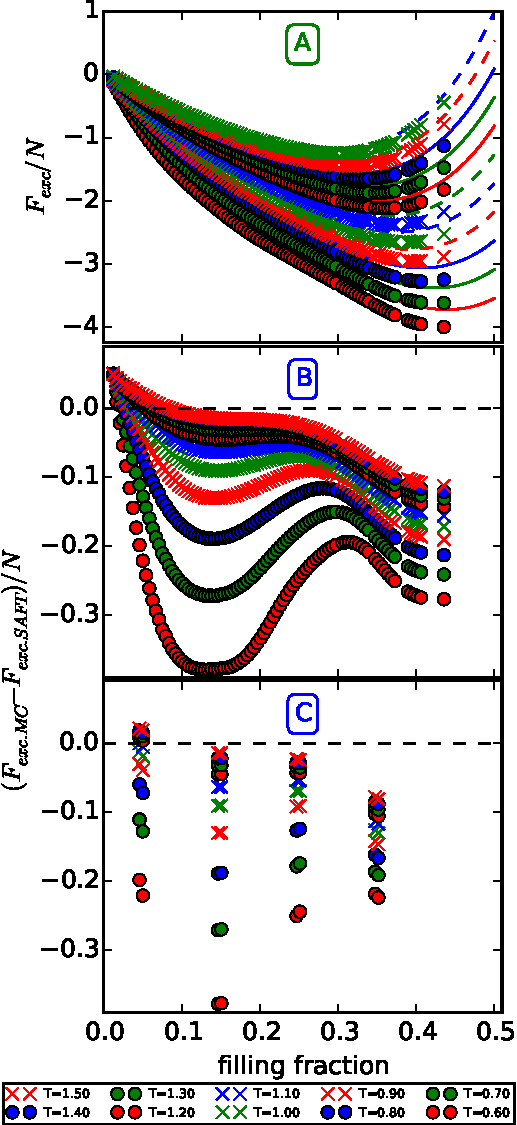
\includegraphics[scale=.9]{FdispVsff-scrunched-ww1.50-L10.00-i0.pdf}
	\caption{\label{fig:FdispVsff}
	\scriptsize \textbf{Here resolution reduction of the data is demonstrated. The data must be generated from a range of box sizes, and for each box size it is possible to run simulations From 2 atoms in a box all the way up to the desired filling fraction of 0.5; depending on the box size, a filling fraction of 0.5 can correspond to only 40 atoms or it could be as much as 100 atoms. Running simulations with every possible filling fraction will indeed produce a nice data set(see figure A), but this will come at the cost of a lengthy computation time. Instead, pairs of simulations are run around filling fractions of [0.5,0.15,0.25,0.35,0.45] (see figure B); the idea is each pair of simulations can be used to interpolate the thermodynamic observables to the selected filling fractions. The comparisons to SAFT are only applied at the selected filling fractions.}}
	
\end{figure}
\vspace*{-10mm}
\subsection{Common Tangent Method}
%\vspace*{-1cm}
\begin{figure}[h!]
\vspace*{-7mm}
\hspace*{-6mm}
	\centering
	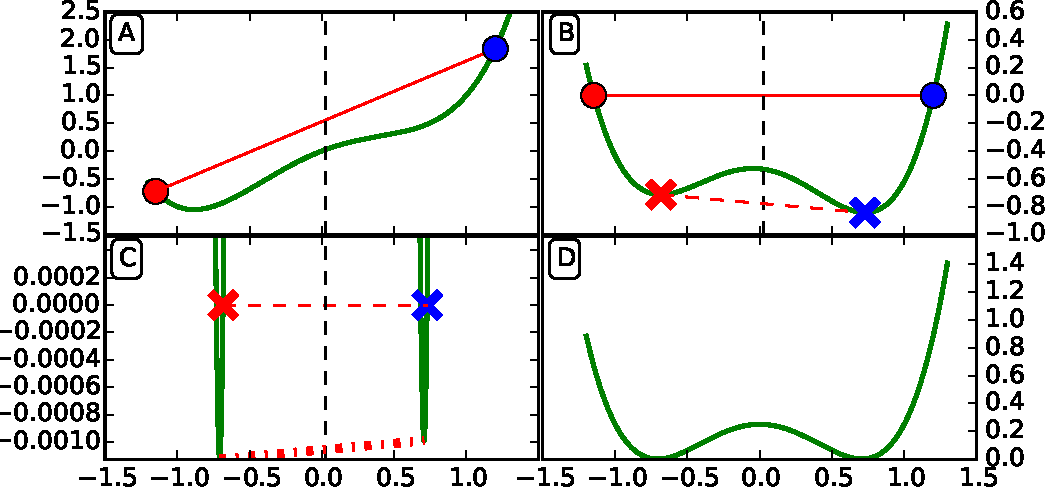
\includegraphics[scale=.9]{pivotMethod.pdf}
	\caption{\label{fig:pivotMethod}
	\scriptsize \textbf{Here the common tangent method is demonstrated. An initial guess value is supplied by the user in plot A as red and blue circles. In plot B all vertical coordinates are taken relative to the red line in plot A; further two new guess values marked as X's are found by taking the minimum on each side of the vertical dashed line in plot B. The dashed line is half way between the guess values in plot A; this vertical line is used to help prevent guess values from jumping across the central bump. The new guess values in plot B are again used to define the vertical coordinates in plot C; the process essentially repeats until the desired accuracy is achieved.}}
	
\end{figure}
\newpage
\vspace*{-7mm}
\subsection{Coexistence points}
\vspace*{-7mm}
\begin{figure}[!h]

\hspace*{-6mm}
	\centering
	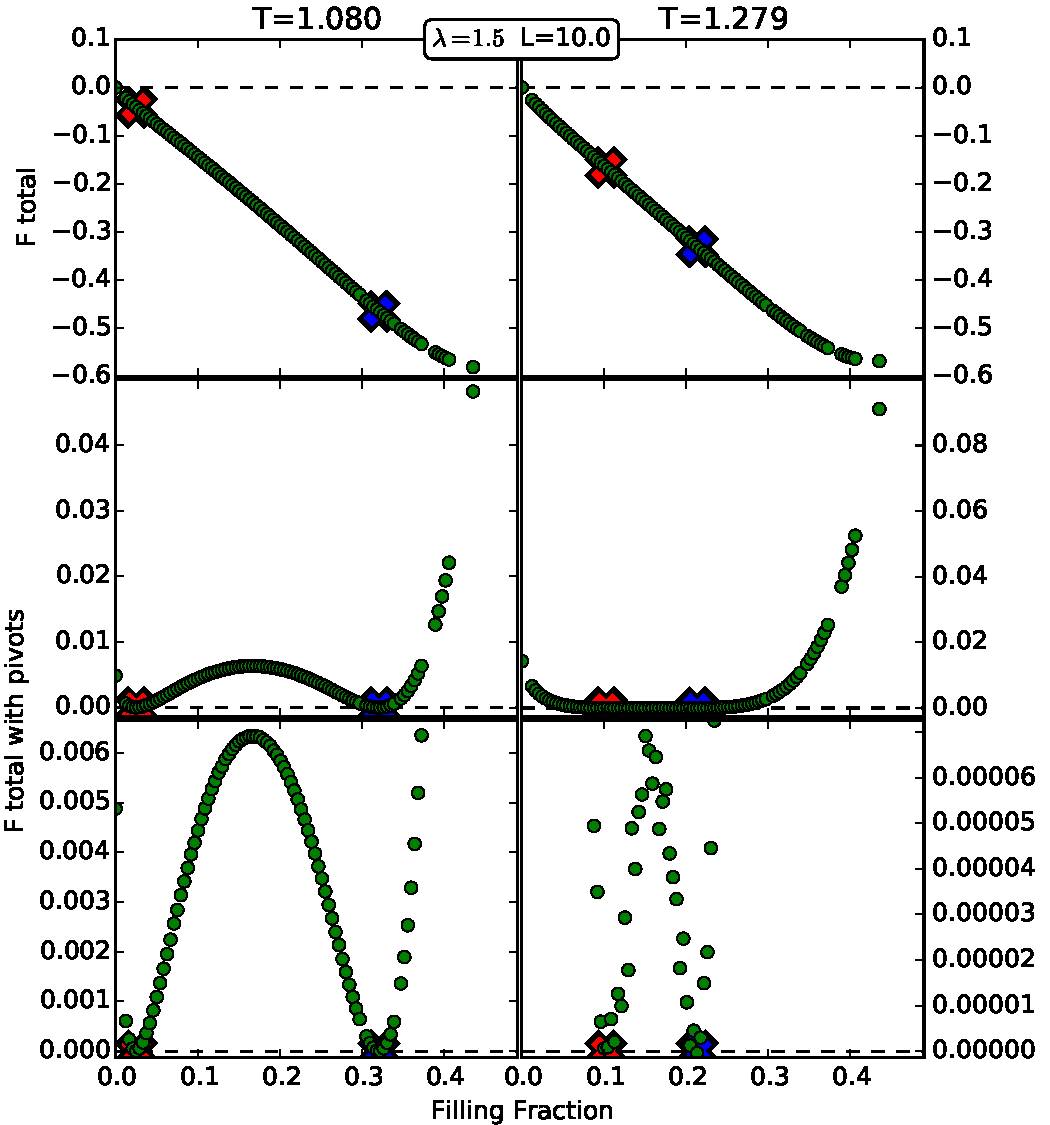
\includegraphics[scale=.9]{commonTangent.pdf}
	\caption{\scriptsize \textbf{Here the common tangent method is applied. The free energy at a particular temperature is plotted as a funciton of density. The two points highlighted by red and blue X's on the curve share a common tangent; this means both points will have the same pressure and chemical potential. The left and right set of plots shows how the signal to noise ratio changes as the temperature increases. Far from the critical point the signal is relatively strong, while the near the critical point the noise becomes significant. To prevent the loss of the signal, first start at a low temperature where the signal is strong. Then gradually increase the temperature while finding common tangents. As the temperature and noise increases, the previous solutions at a slightly lower temperature can be used as a guess for the new higher temperature.}}
	\label{fig:FdispVsff}
\end{figure}




%\pagestyle{fancy}   % Reset all pages after this file to fnacy headers

\chapter{Results}
%\renewcommand{\chaptermark}{ HI}
\stepcounter{subsection}
\addcontentsline{toc}{subsection}{\protect\numberline{\thesubsection}<Monte Carlo Energy trends>}
\begin{figure}[h]
\vspace*{-10mm}
\hspace*{-6mm}
	\centering
	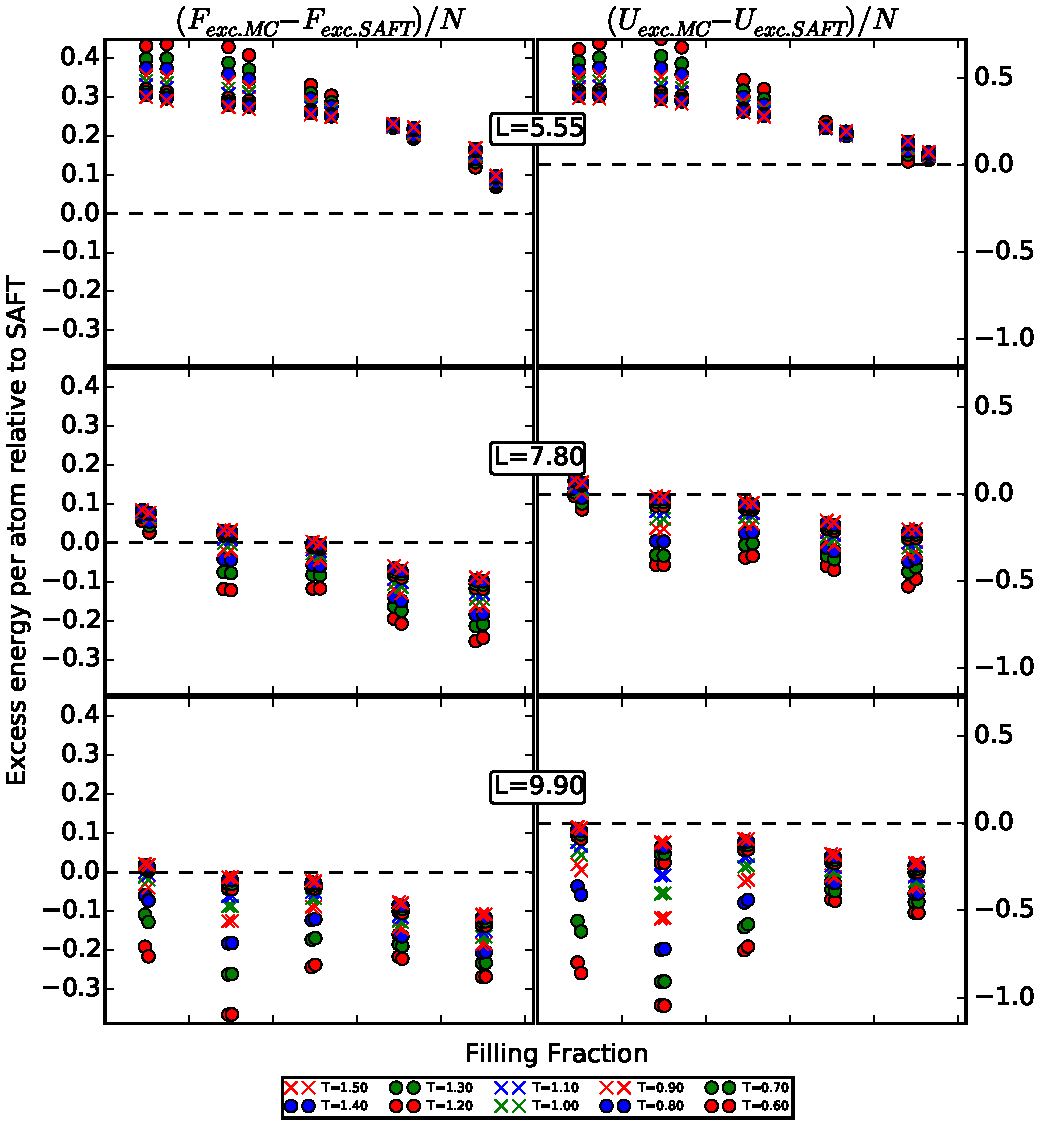
\includegraphics[scale=.9]{UFtrends-ww1.50.pdf}
	\caption{
	%\tiny	
	\scriptsize
	These graphs show the Monte Carlo simulation results in terms of dispersive free energy and internal energy relative to SAFT at three different box sizes. Both sets of graphs show that a small box size has a higher energy than SAFT, while a larger box will have a lower energy than SAFT. This makes sense because as the box size increases longer wavelength fluctuations are allowed, and these longer wavelengths actually lower the allowed energy as the increase in energy due to the low density regions are more than compensated by the decrease in energy due to the high density regions. Given a constant box size, the high filling fraction simulations cannot fluctuate as much as the low filling fraction simulations, which explains the bulge in the two lower plots.}
	\label{fig:UFtrends}
\end{figure}
%And also a citation example \cite{Forte2011}.
%And this one too \cite{Forte2013}


\pagebreak
\begin{figure}[h]
\vspace*{-7mm}
\hspace*{-6mm}
	\centering
	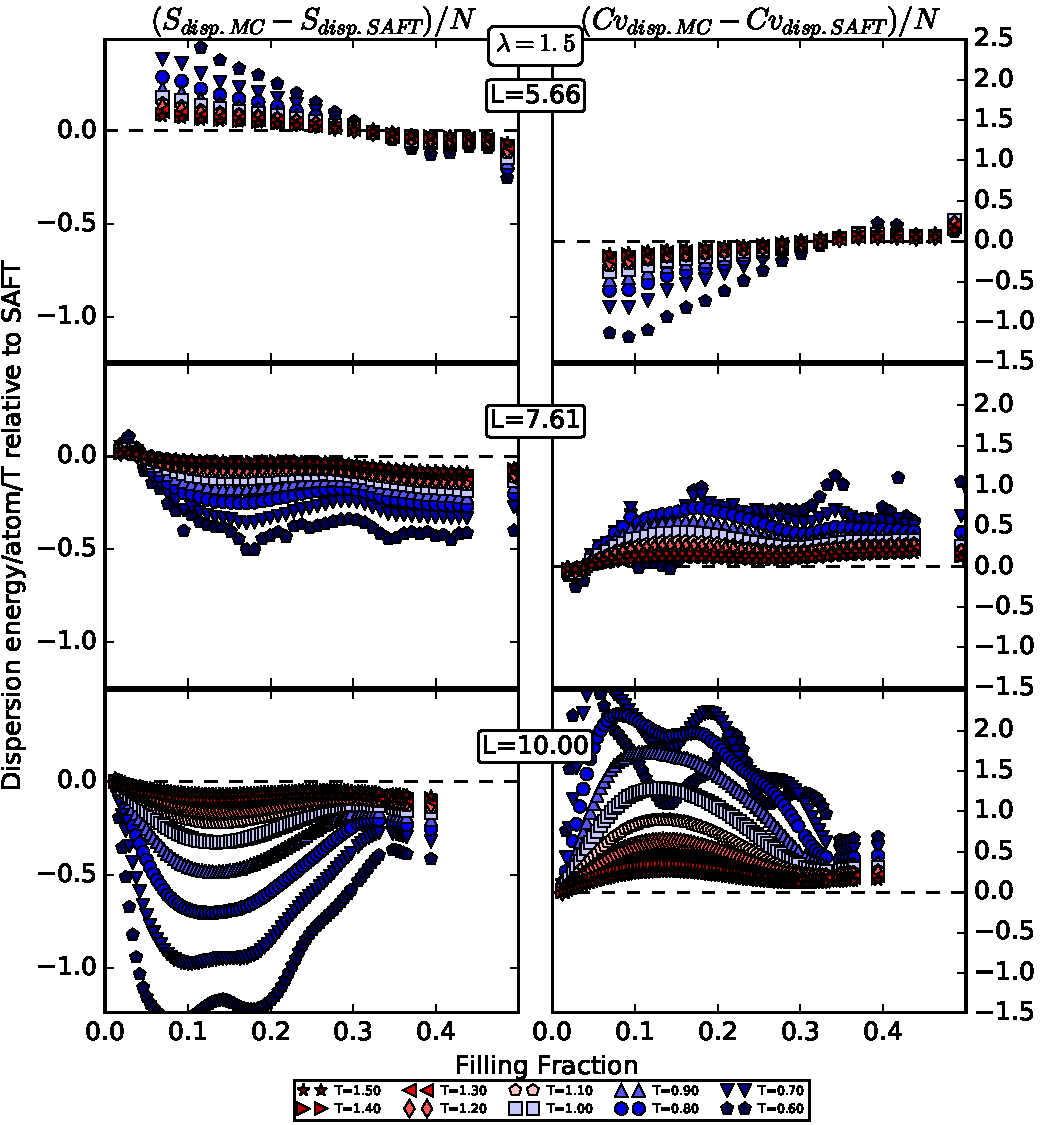
\includegraphics[scale=.9]{STCvtrends-ww1.50.pdf}
	\caption{\scriptsize
	These graphs show the Monte Carlo simulations results in terms of dispersive entropy and heat capacity per particle relative to SAFT at three different box sizes. It is interesting to see the entropy trends are nearly the inverse of the heat capacity trends. Both entropy and heat capacity require a derivative to find, it is just that entropy is the negative derivative of Free energy while heat capacity is the positive derivative of internal energy. Given fig. \ref{fig:UFtrends} showed the internal energy had the same trend as the free energy, it isn't surprising entropy and heat capacity have inverse trends. Regarding the trend itself, the entropy of a small box will have more entropy than SAFT, while a large box will have a lower entropy than SAFT. This trend can be explained by the particles binding together in ways that SAFT could not take into account, and this extra binding will decrease the entropy simply because some states are now favored over other states.}
	\label{fig:STCvtrends}
\end{figure}


\pagebreak
\begin{figure}[h]
\vspace*{-7mm}
\hspace*{-6mm}
	\centering
	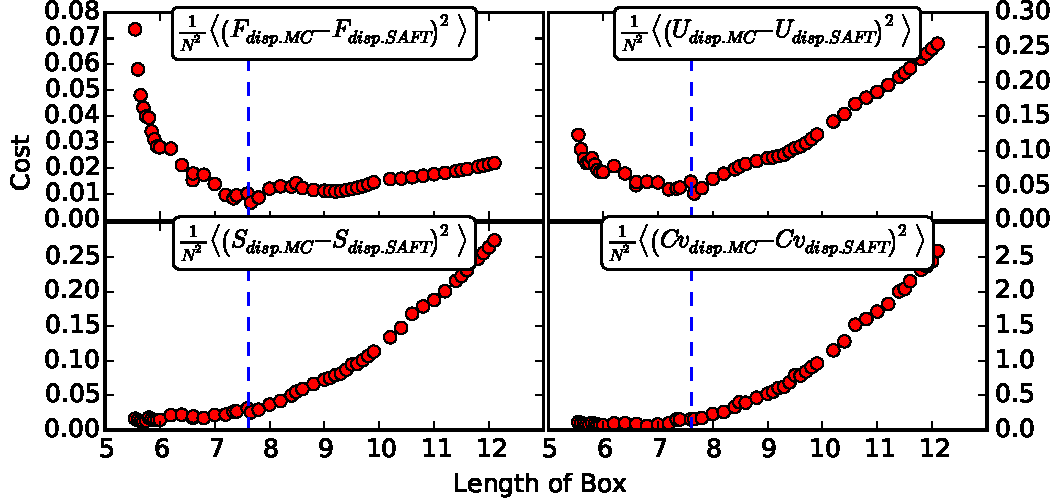
\includegraphics[scale=.9]{Costsmall-ww1.50.pdf}
	\caption{\scriptsize
	These graphs show the cost function as a function of the box size for the dispersive free energy, internal energy, entropy, and heat capacity. The cost function is defiend as the mean square difference between the Monte Carlo simultions and SAFT evaulated at a filling fraction of [0.15,0.25,0.35,0.45] and evaluated for 0.6\textless T\textless 1.5. The dispersive free energy and internal energy show a minimum near L=7.6, while any box size less than L=8.0 seems to be just fine for the dispersive entropy and heat capacity.}
	\label{fig:Cost}
\end{figure}
\begin{figure}[h]
\vspace*{-7mm}
\hspace*{-6mm}
	\centering
	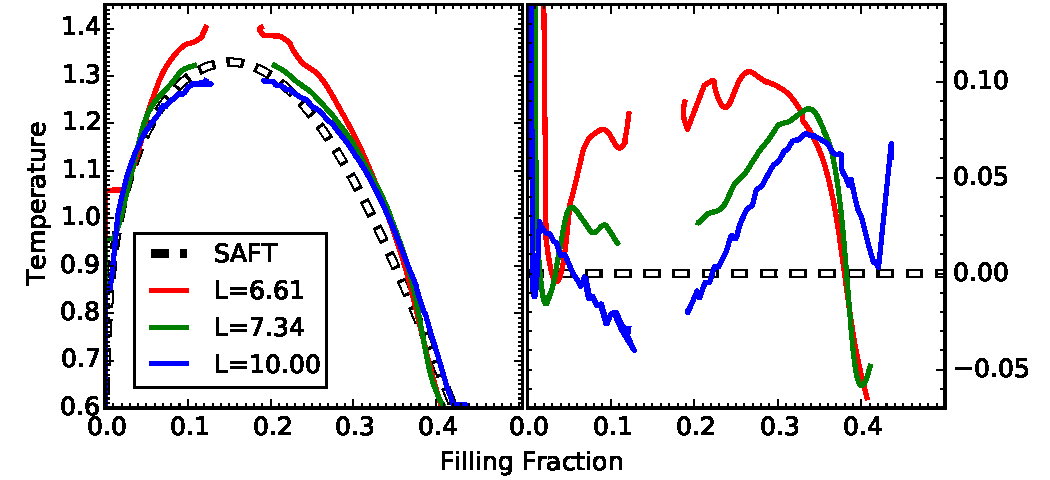
\includegraphics[scale=0.9]{coexistence-ww1.50.pdf}
	\caption{\scriptsize
	Here the gas-liquid coexistence temperature as a function of filling fraction for three different Monte Carlo simulations are compared to SAFT. The box size L=6.61 clearly has a higher critical temperature than SAFT, while the box size L=10.0 clearly has a lower critical temperature than SAFT.}
	\label{fig:Coexistence}
\end{figure}





%\chapter{Data}
%\section{Computation}

Provide computation methods and data of what I have done so far.

This is how you can refer to fig \ref{fig:liq vap co}. % Note: Have to build the latex document twice for it to work.


%sample image input
\begin{figure}[h]
	\centering
	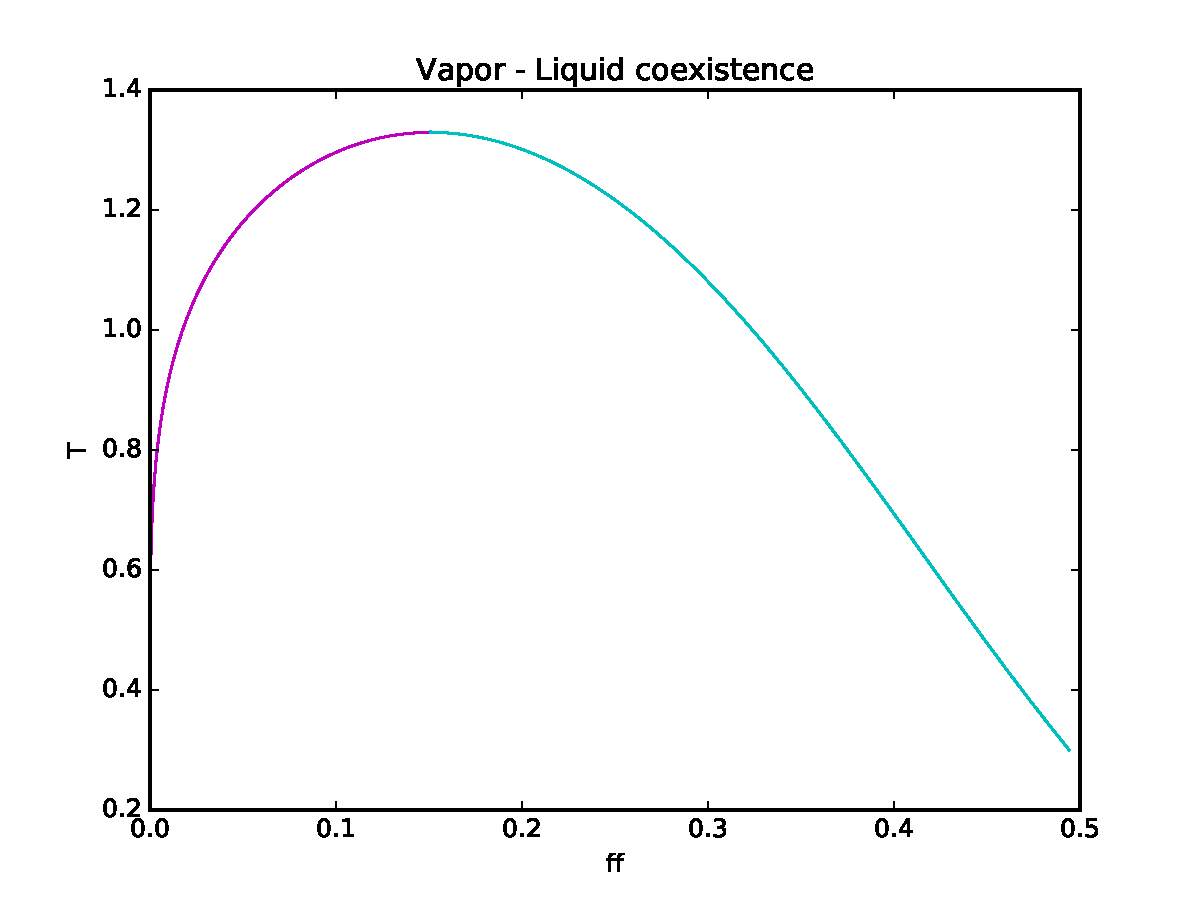
\includegraphics[scale=0.5]{liqVapCo_Tvsff}
	\caption{Caption for this image.}
	\label{fig:liq vap co}
\end{figure}

%sample multi image input
\begin{figure}[h]
	\centering
	\begin{subfigure}[b]{0.3\textwidth}
	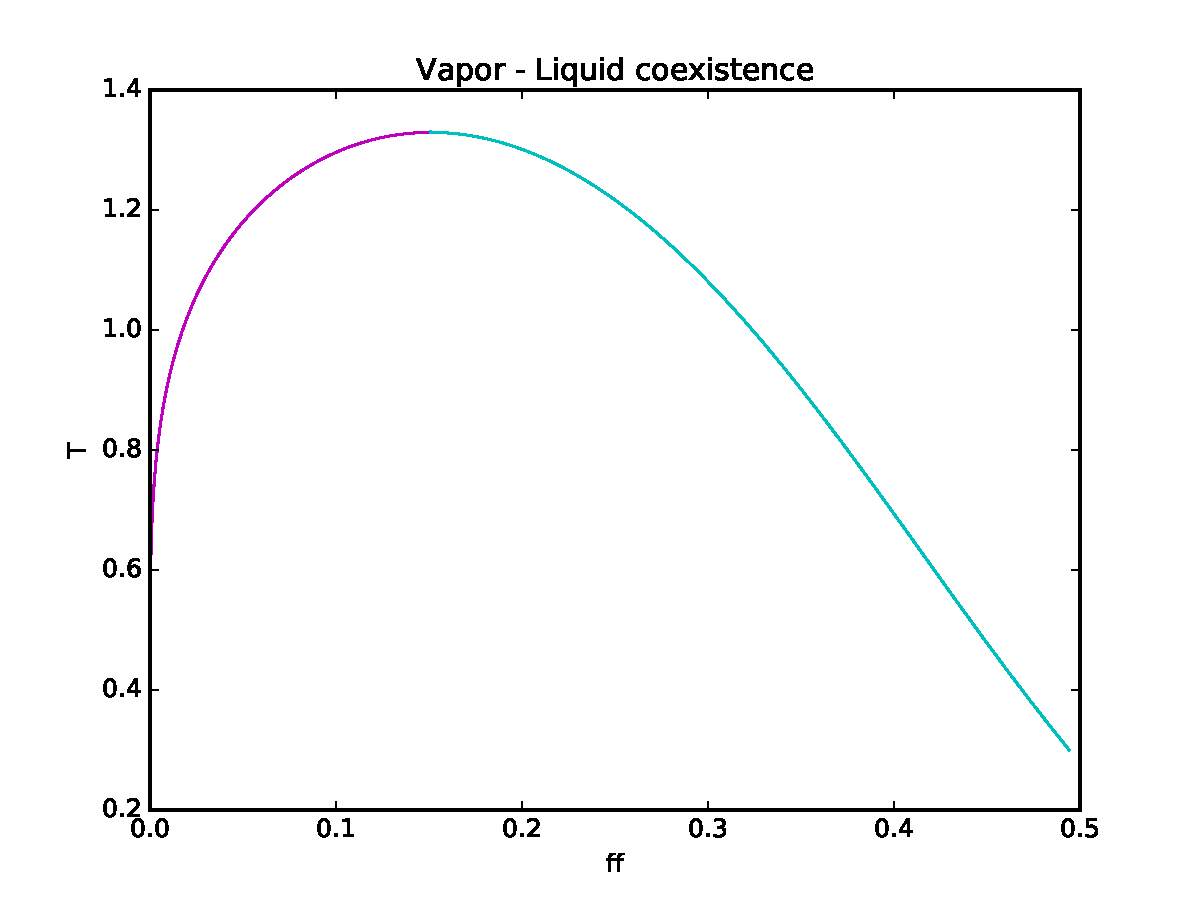
\includegraphics[width=\textwidth]{liqVapCo_Tvsff}
	\caption{Caption 01}
	\label{fig:cap01}
	\end{subfigure}
	\hfill
	\begin{subfigure}[b]{0.3\textwidth}
	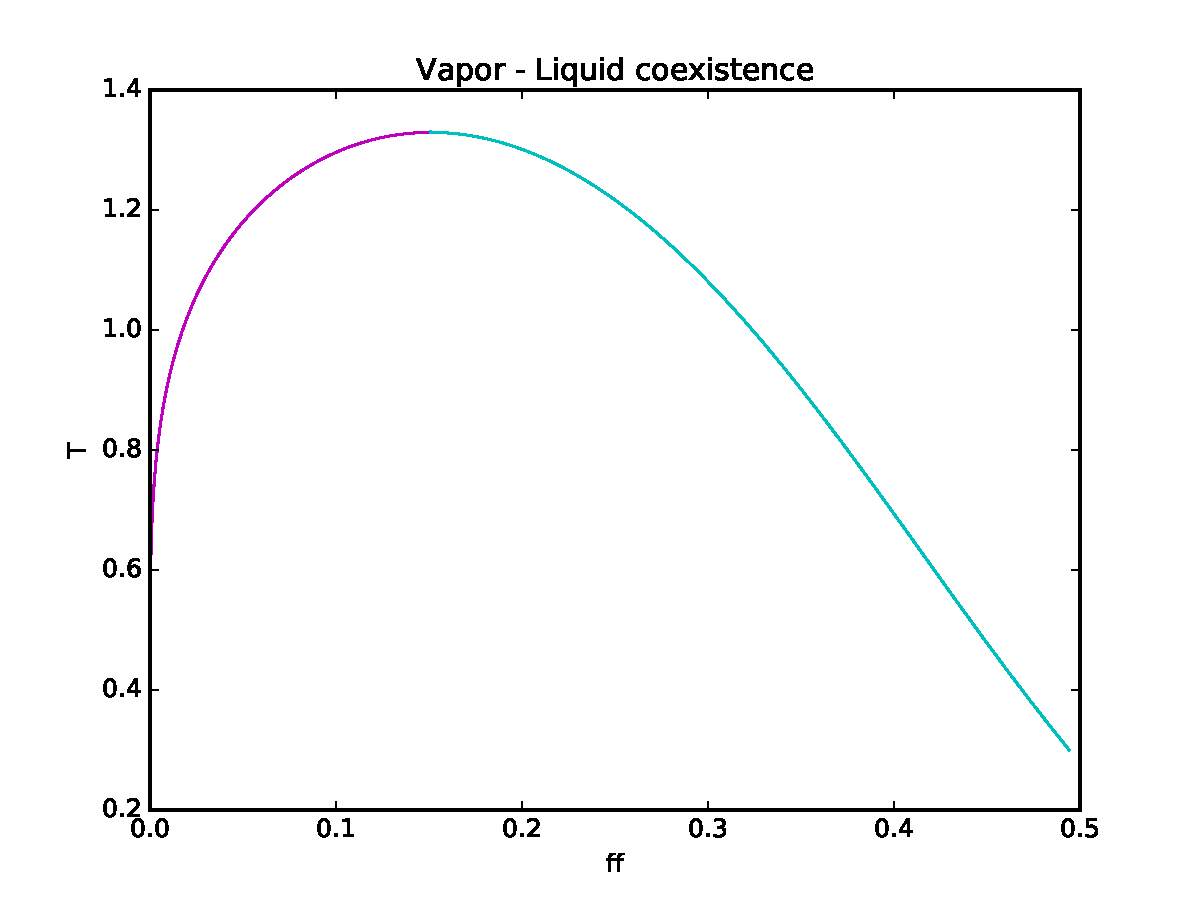
\includegraphics[width=\textwidth]{liqVapCo_Tvsff}
	\caption{Caption 02}
	\label{fig:cap01}
	\end{subfigure}
	\hfill
	\begin{subfigure}[b]{0.3\textwidth}
	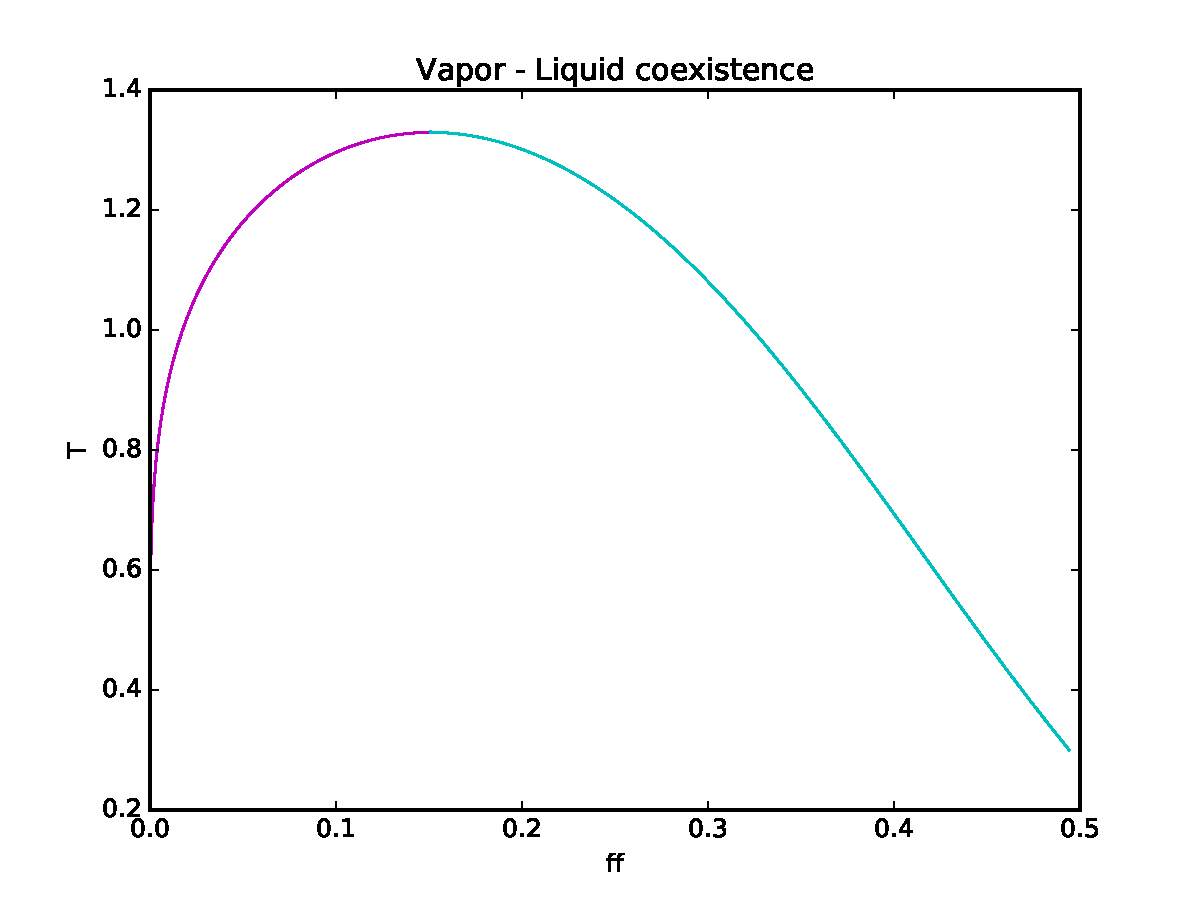
\includegraphics[width=\textwidth]{liqVapCo_Tvsff}
	\caption{Caption 03}
	\label{fig:cap01}
	\end{subfigure}
	\caption{Caption for all three.}
	\label{fig:cap123}
\end{figure}

\chapter{Conclusion}
\section{Conclusion}
SAFT uses perturbation to incorporate interactions up to some unknown length scale L. GRG builds upon SAFT by incorporating even longer wavelengths in an iterative manner. Unfortunately the unknown length scale is a free parameter. Free parameters are usually varied to find the best fit with experiment, but extra free parameters that aren't needed usually saps a model of its predictive abilities. In the extreme case, a bunch of experiments can be interpolated to 'predict' what will happen in the valid range of the data, yet the interpolation will fail far from the actual data. This failure to make predictions can also happen to models with too many free parameters which is undesirable for everyone involved.

This project explored how to fix the arbitrary parameter L in GRG by instead comparing the results of Monte Carlo simulations to SAFT. Given that SAFT only incorporates interactions up to some length scale L, the Monte Carlo simulations with a box size of length L should be able to reproduce the results of SAFT. This project did vary the box size of the Monte Carlo simulations and found a 'best' fit length of roughly L=(7.6). To test this best fit, the phase coexistence was found for three box sizes and compared to SAFT. Boxes much smaller than 7.6 had a critical point higher than SAFT, while box sizes much larger than 7.6 had a critical point below SAFT.

While working on this project, I honestly thought the noise of the simulations would drown out the coexistence points. It was interesting to see the coexistence plots actually see a signal as low as (0.00006) (see fig~\ref{fig:FdispVsff}). Work for the future would include running multiple simulations to increase the signal to noise ratio, auto detection of outliers, and finally a comparison using GRG with L=10.0 and L=7.61.


\printbibliography

\end{document}